
\documentclass[11pt]{article}
\usepackage[margin=1in]{geometry}
\usepackage{amsmath,amssymb,booktabs,array,longtable}
\usepackage{graphicx}
\usepackage{hyperref}
\usepackage{enumitem}
\usepackage{titlesec}
\usepackage{float}

\begin{document}

\begin{center}
\Large\textbf{Shiv Nadar University Chennai}\\[2mm]
\end{center}

\renewcommand{\arraystretch}{1.4}

\begin{flushleft}
\textbf{Name:} Johan Emmanuel S\\
\textbf{Registration Number:} 24011101043\\
\end{flushleft}

\begin{tabular}{|p{3.5cm}|p{8cm}|p{2cm}|}
\hline
Degree \& Branch & B.Tech Artificial Intelligence \& Data Science & Semester V\\ \hline
Subject Code \& Name & CS3807 -- Deep Learning Laboratory & AY: 2026--27\\ \hline
\end{tabular}

\vspace{3mm}

\begin{center}
\Large\textbf{Experiment 1}\\
\large\textbf{Implementation of a Single Layer Perceptron for Binary Classification}
\end{center}

%----------------------------------------------------------

\section*{1. Objective}

The objective of this experiment is to understand the concept of an artificial neuron and implement a Single Layer Perceptron from scratch for binary classification. Students will learn the perceptron learning algorithm, understand the importance of activation functions, visualize the learning process, and evaluate the classifier using a real-world dataset.

%----------------------------------------------------------

\section*{2. Background Theory}

An Artificial Neuron is the fundamental building block of a neural network. It receives one or more input features, multiplies them by corresponding weights, adds a bias term, and applies an activation function to determine the output.

The Single Layer Perceptron is the earliest supervised learning algorithm capable of solving linearly separable binary classification problems.

\subsection*{Mathematical Formulation}

Weighted Sum

\[
z=\mathbf{w}^{T}\mathbf{x}+b
\]

where

\begin{itemize}
\item $\mathbf{x}$ : Input vector
\item $\mathbf{w}$ : Weight vector
\item $b$ : Bias
\item $z$ : Linear combination
\end{itemize}

Prediction

\[
\hat y=f(z)
\]

Weight Update Rule

\[
\mathbf{w}_{new}
=
\mathbf{w}_{old}
+
\eta
(y-\hat y)
\mathbf{x}
\]

Bias Update

\[
b_{new}
=
b_{old}
+
\eta
(y-\hat y)
\]

where $\eta$ denotes the learning rate.

%----------------------------------------------------------

\section*{3. Activation Functions}

An activation function determines the output of a neuron based on the weighted sum of its inputs. It introduces non-linearity, enabling neural networks to learn complex patterns. Although the perceptron uses only the Step Activation Function, modern deep learning models employ differentiable activation functions for efficient optimization through backpropagation.

\subsection*{Step Activation Function}

\[
f(z)=
\begin{cases}
1,&z\ge0\\
0,&z<0
\end{cases}
\]

The Step Activation Function produces a binary output and is therefore suitable only for linearly separable binary classification problems.

\begin{center}
\begin{tabular}{|p{2.5cm}|p{3cm}|p{6cm}|}
\hline
\textbf{Activation} & \textbf{Output Range} & \textbf{Typical Applications}\\
\hline
Step & $\{0,1\}$ & Classical Perceptron\\
\hline
Sigmoid & $(0,1)$ & Binary Classification Output Layer\\
\hline
Tanh & $(-1,1)$ & Hidden Layers (Traditional Networks)\\
\hline
ReLU & $[0,\infty)$ & Hidden Layers in CNNs and MLPs\\
\hline
Leaky ReLU & $(-\infty,\infty)$ & Avoiding Dying ReLU\\
\hline
Softmax & $(0,1)$ & Multi-class Classification Output Layer\\
\hline
\end{tabular}
\end{center}

\textbf{Note:} This experiment uses only the Step Activation Function. The remaining activation functions will be studied in subsequent experiments involving Multilayer Perceptrons and Deep Neural Networks.

%----------------------------------------------------------

\section*{4. Dataset Description}

\textbf{Dataset:} Banknote Authentication Dataset

\textbf{Source:} UCI Machine Learning Repository

\textbf{Download Link:}

\url{https://archive.ics.uci.edu/dataset/267/banknote+authentication}

\begin{center}
\begin{tabular}{|l|l|}
\hline
Instances & 1372\\
\hline
Features & 4 Numerical Features\\
\hline
Classes & 2\\
\hline
Missing Values & None\\
\hline
Task & Binary Classification\\
\hline
\end{tabular}
\end{center}

\textbf{Feature Description}

\begin{itemize}
\item Variance
\item Skewness
\item Curtosis
\item Entropy
\end{itemize}

Target Class

\begin{itemize}
\item 0 -- Authentic Banknote
\item 1 -- Forged Banknote
\end{itemize}

%----------------------------------------------------------

\section*{5. Experimental Procedure}

\textbf{Task 1: Dataset Exploration}

\begin{itemize}
\item Load the dataset.
\item Display the first five samples.
\item Determine dataset dimensions.
\item Identify missing values.
\item Display descriptive statistics.
\end{itemize}

\vspace{2mm}

\textbf{Task 2: Exploratory Data Analysis}

Generate

\begin{itemize}
\item Histograms
\item Correlation Heatmap
\item Scatter Plot
\item Boxplots
\end{itemize}

\vspace{2mm}

\textbf{Task 3: Data Preprocessing}

\begin{itemize}
\item Normalize all numerical features.
\item Split the dataset into Training (80\%) and Testing (20\%).
\end{itemize}

\vspace{2mm}

\textbf{Task 4: Perceptron Implementation}

Implement from scratch

\begin{itemize}
\item Weight Initialization
\item Bias Initialization
\item Step Activation Function
\item Forward Propagation
\item Perceptron Learning Rule
\end{itemize}

\vspace{2mm}

\textbf{Task 5: Model Training}

Display

\begin{itemize}
\item Epoch Number
\item Misclassified Samples
\item Updated Weights
\item Updated Bias
\end{itemize}

\vspace{2mm}

\textbf{Task 6: Model Evaluation}

Compute

\begin{itemize}
\item Accuracy
\item Precision
\item Recall
\item F1-score
\item Confusion Matrix
\end{itemize}

%----------------------------------------------------------

\section*{7. Source Code}
The code for the Single Layer Perceptron with the data processing and analysis can be found at \url{https://github.com/faultybyte/deep-learning-lab}

%----------------------------------------------------------

\section*{8. Experimental Results}

\subsection*{Model Performance Evaluation}
The Single Layer Perceptron was evaluated on the unseen testing dataset (20\% split). The standard classification performance metrics computed from the confusion matrix are as follows:
\begin{itemize}
    \item \textbf{Classification Accuracy:} 0.9927
    \item \textbf{Precision:} 1.0000
    \item \textbf{Recall (Sensitivity):} 0.9843
    \item \textbf{F1-score:} 0.9921
\end{itemize}

\subsection*{Model Parameter Validation}
Upon convergence, the final internal parameters learned by the Perceptron is given below:
\begin{itemize}
    \item \textbf{Final Weight Vector ($\mathbf{w}$):} $[-0.16, -0.16, -0.18, 0.01]$
    \item \textbf{Final Scalar Bias ($b$):} 0.21
\end{itemize}

%----------------------------------------------------------

\section*{9. Generated Plots and Interpretations}

\subsection*{Exploratory Data Analysis (EDA) Visualizations}

\begin{figure}[H]
    \centering
    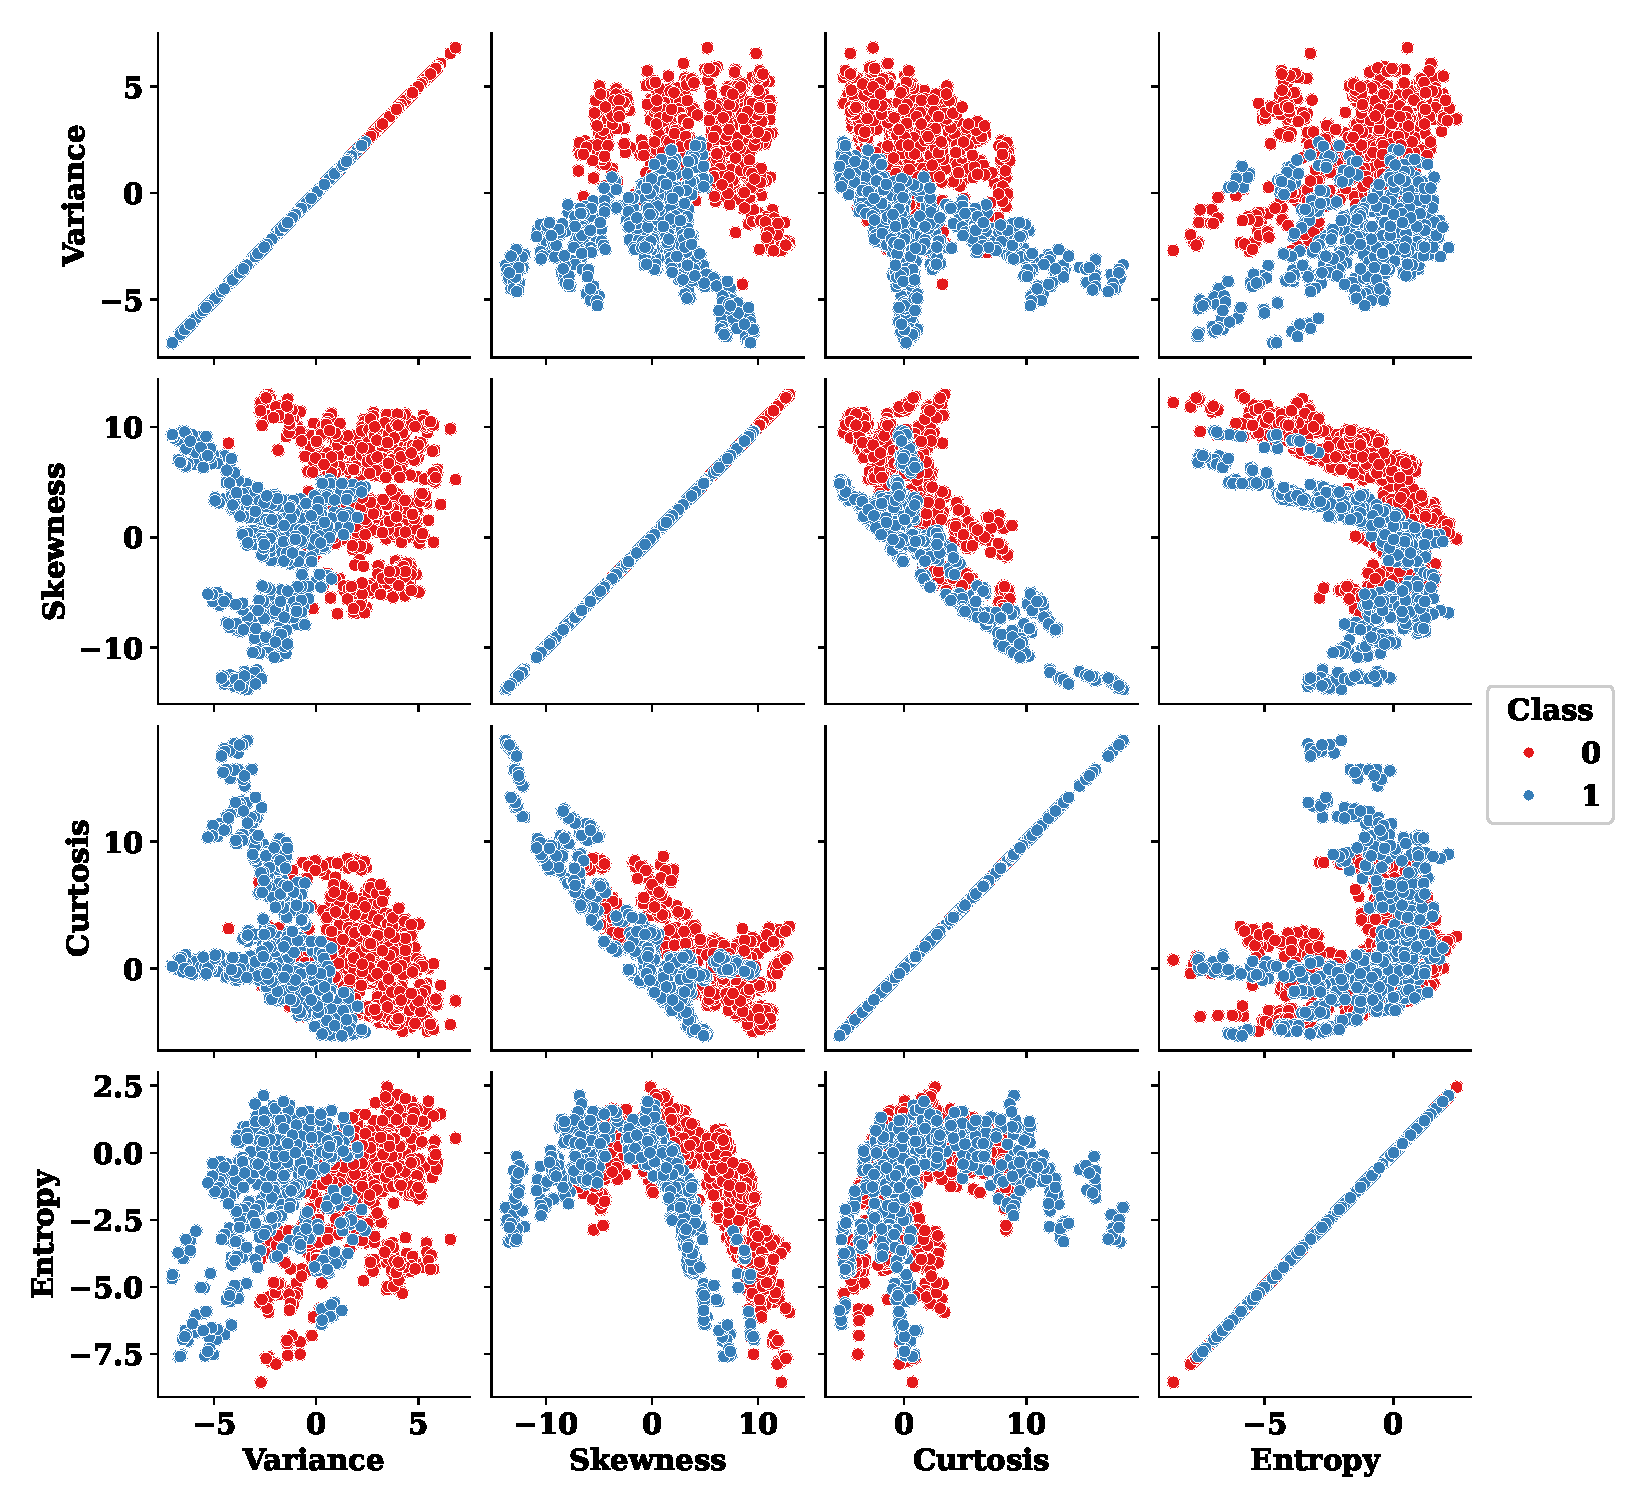
\includegraphics[width=0.7\textwidth]{banknote_pairplots.eps}
    \caption{Pairwise Scatter Plot Matrix of Banknote Features.}
    \label{fig:pairplot}
\end{figure}
\textbf{Interpretation:} For most pairs of features, the classes can be separated using a straight line. But they are not fully linearly separable, hence the perceptron will not converge but will still yield high accuracy.

\begin{figure}[H]
    \centering
    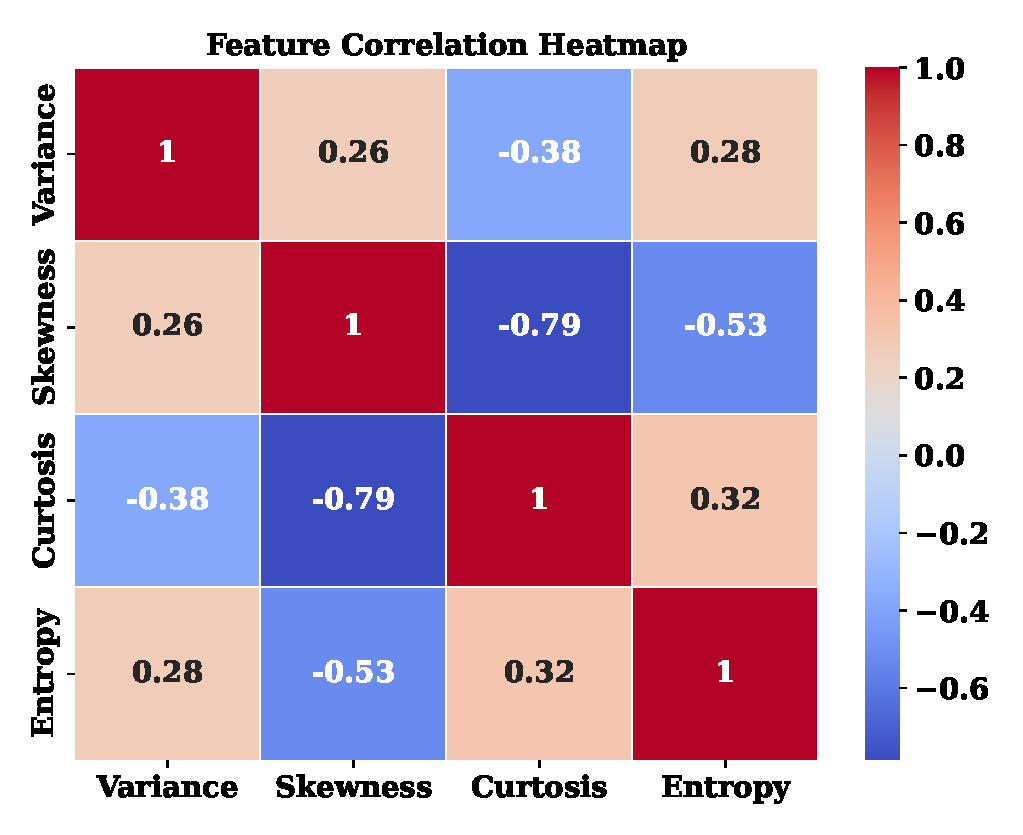
\includegraphics[width=0.7\textwidth]{banknote_heatmap.eps}
    \caption{Feature Correlation Heatmap of Banknote Features.}
    \label{fig:heatmap}
\end{figure}
\textbf{Interpretation:} Skewness and Curtosis, Variance and Curtosis are negatively correlated, all other feature pairs are positively correlated.

\begin{figure}[H]
    \centering
    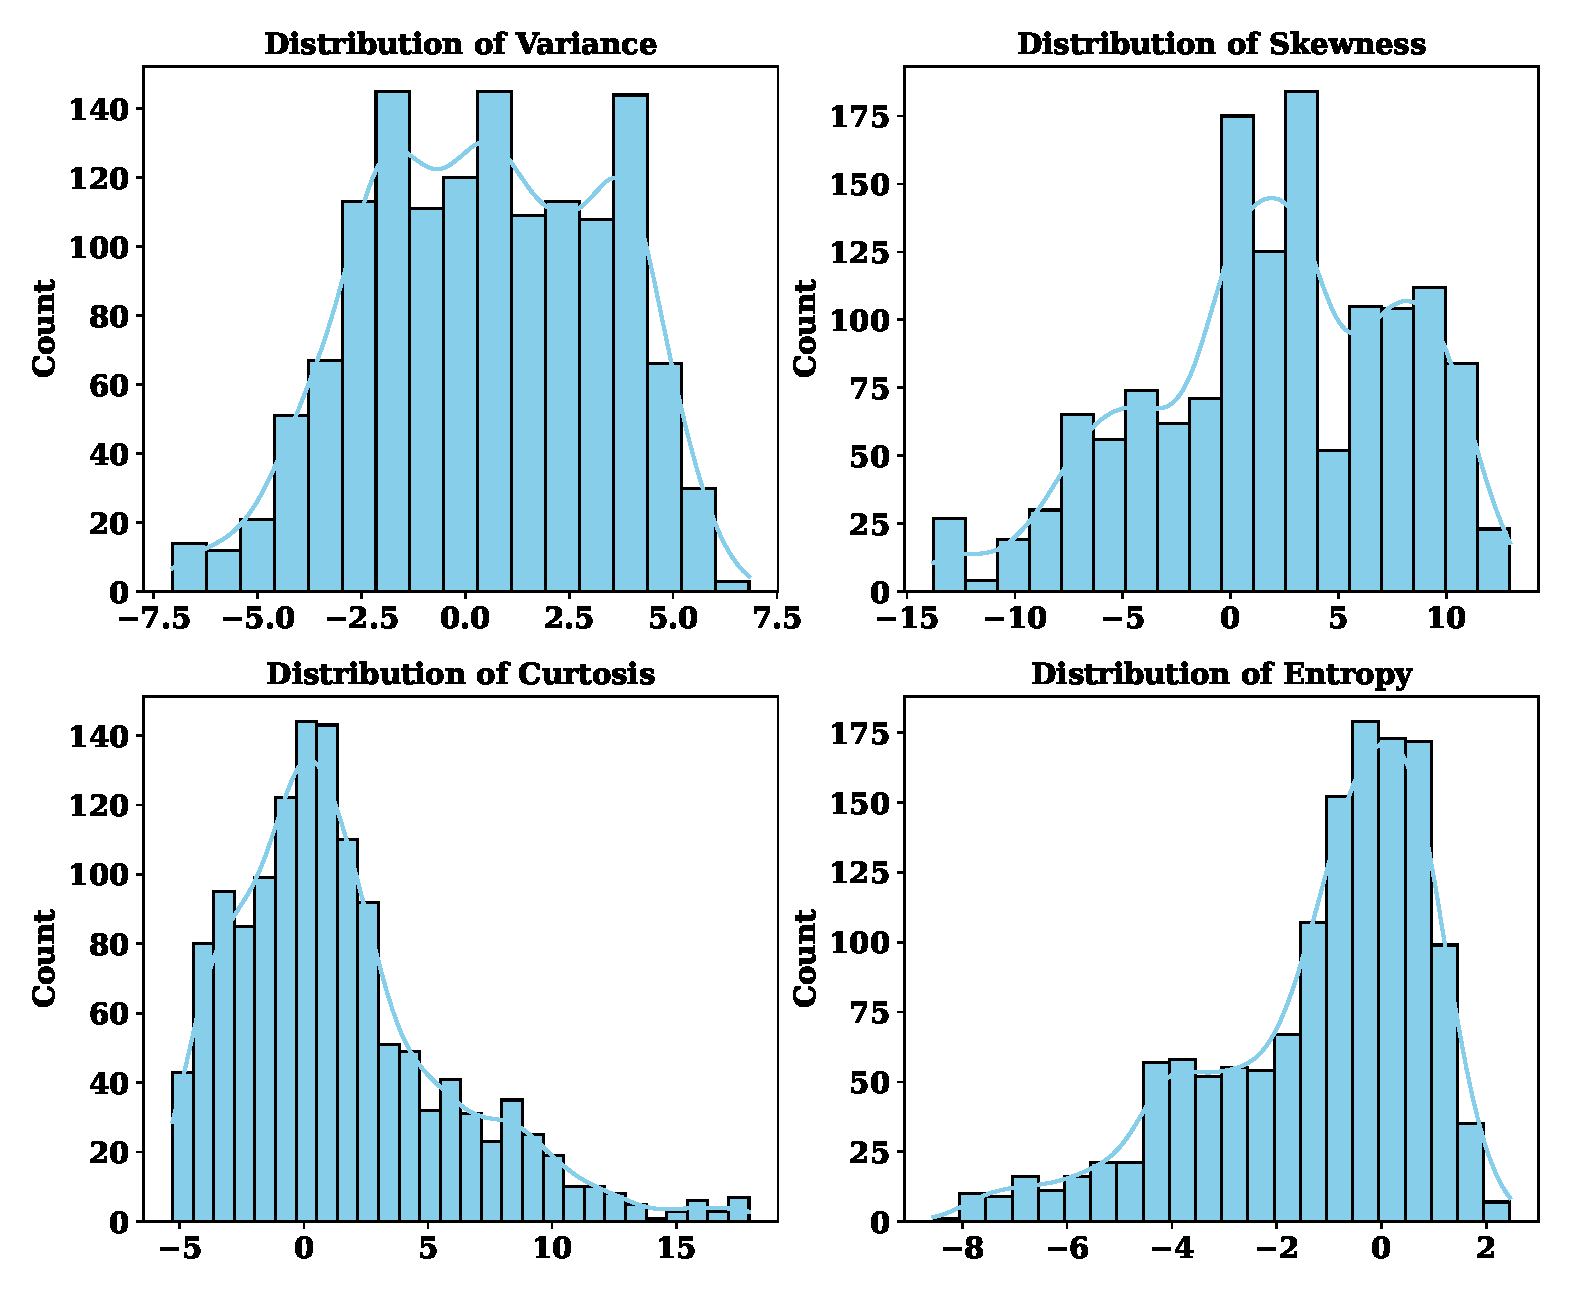
\includegraphics[width=0.7\textwidth]{banknote_histograms.eps}
    \caption{Feature Distribution via Feature Histograms.}
    \label{fig:histograms}
\end{figure}
\textbf{Interpretation:} Variance and Skewness are almost normally distributed but are composed of individual Gaussian curves. Curtosis is right skewed and Entropy is left skewed. 

\begin{figure}[H]
    \centering
    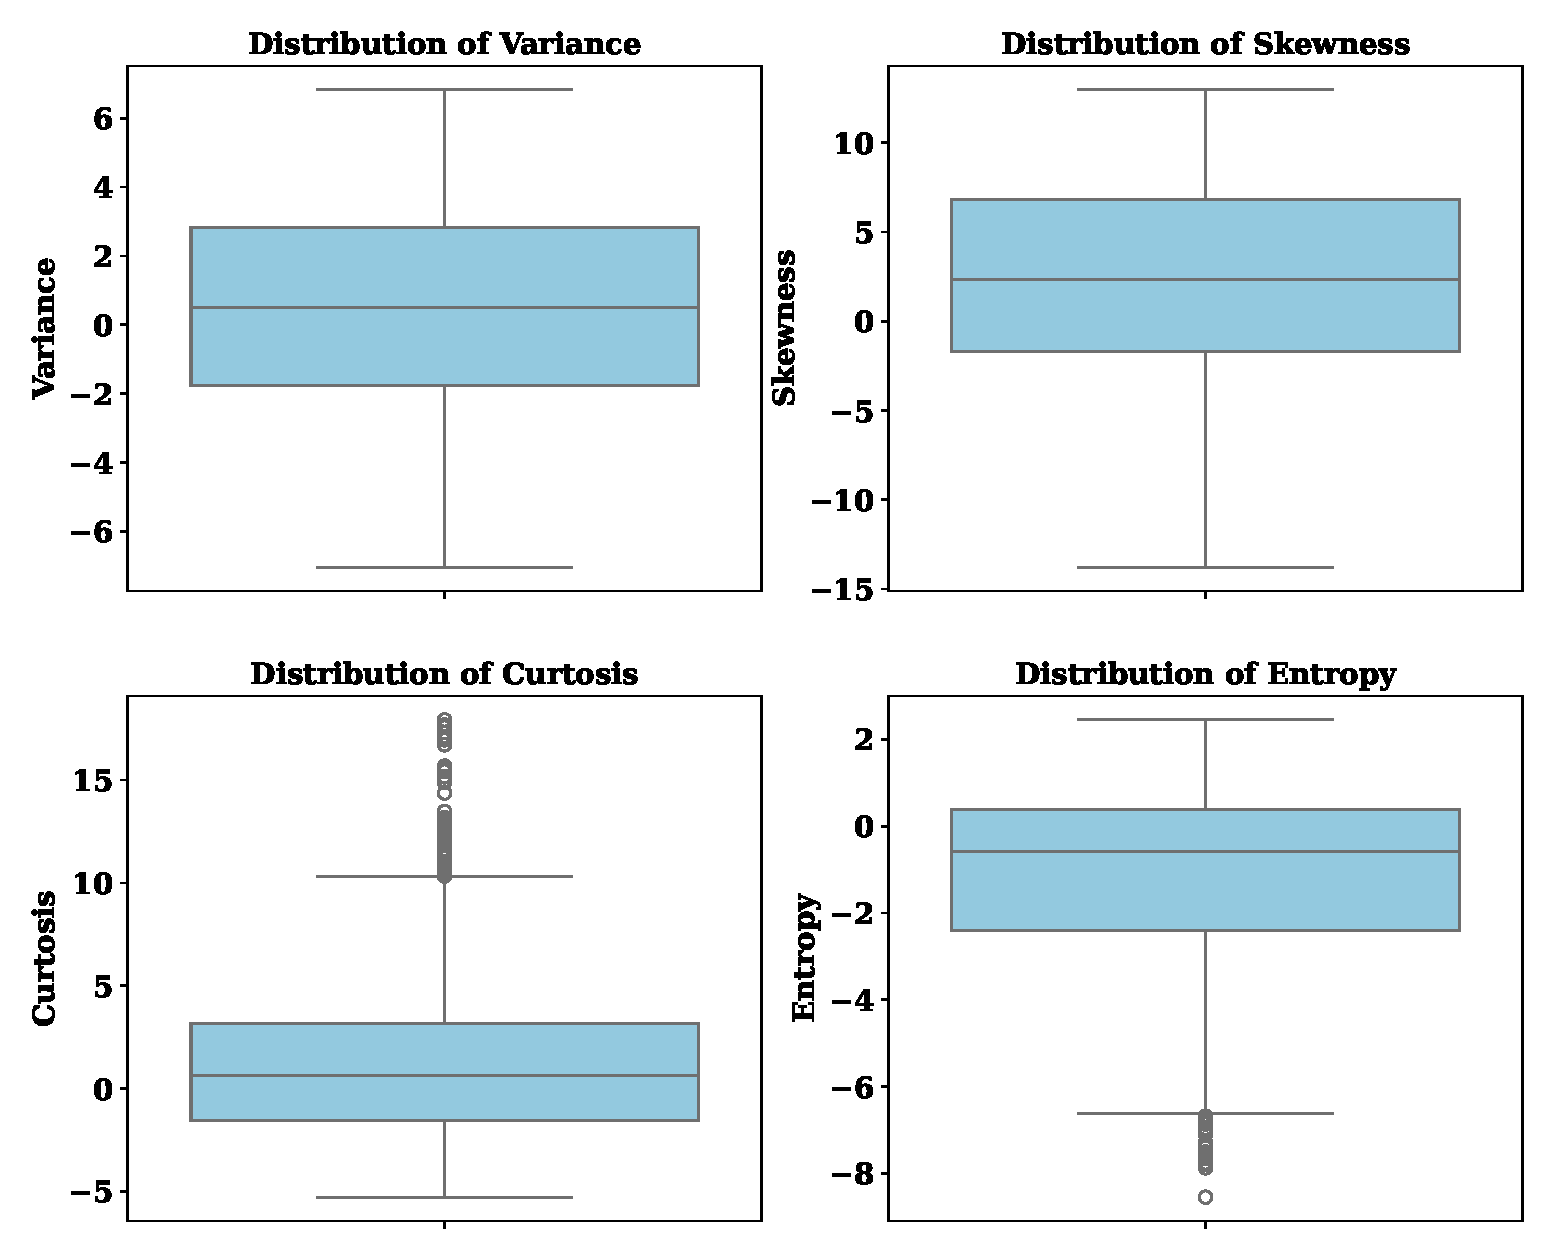
\includegraphics[width=0.7\textwidth]{banknote_boxplots.eps}
    \caption{Feature Distribution and Outlier Analysis via Boxplots.}
    \label{fig:boxplots}
\end{figure}
\textbf{Interpretation:} Variance and Skewness have no outliers while Entropy and Curtosis have outliers that fall over the standard normal range.

\subsection*{Optimization and Parameter Convergence Plots}

\begin{figure}[H]
    \centering
    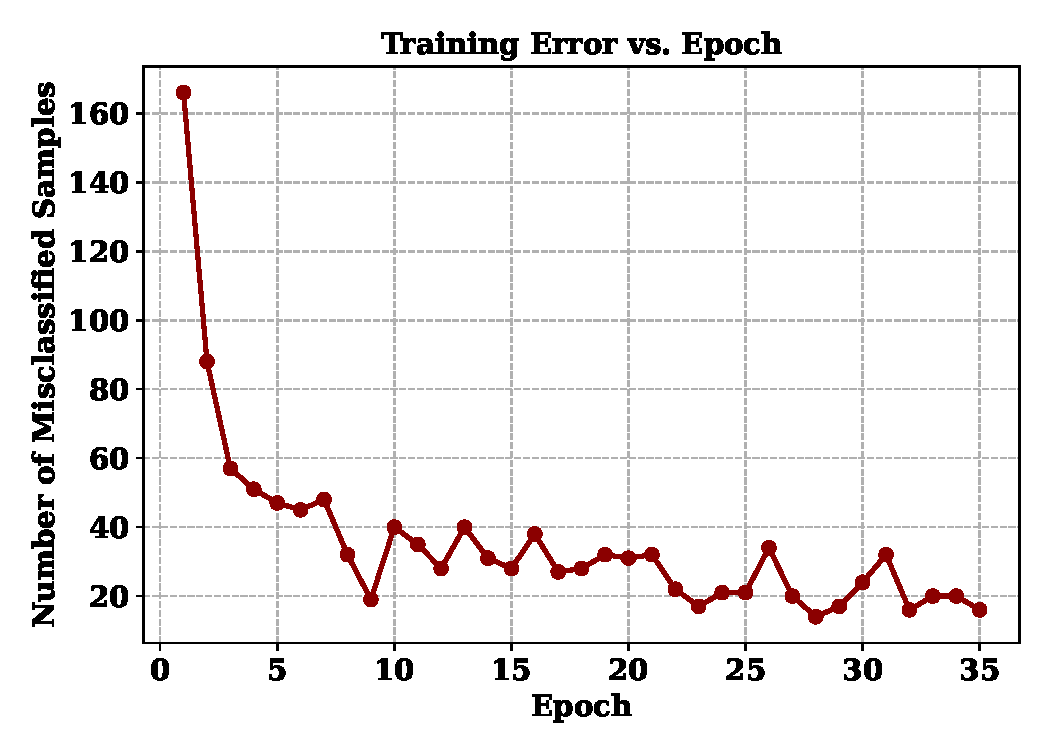
\includegraphics[width=0.7\textwidth]{error_vs_epoch.eps}
    \caption{Training Error Convergence Profile Across Epochs.}
    \label{fig:error_convergence}
\end{figure}
\textbf{Interpretation:} The error drastically reduces in the first five epochs, however it fluctuates but never touches zero, because the perceptron could not converge as the data is not fully linearly separable.

\begin{figure}[H]
    \centering
    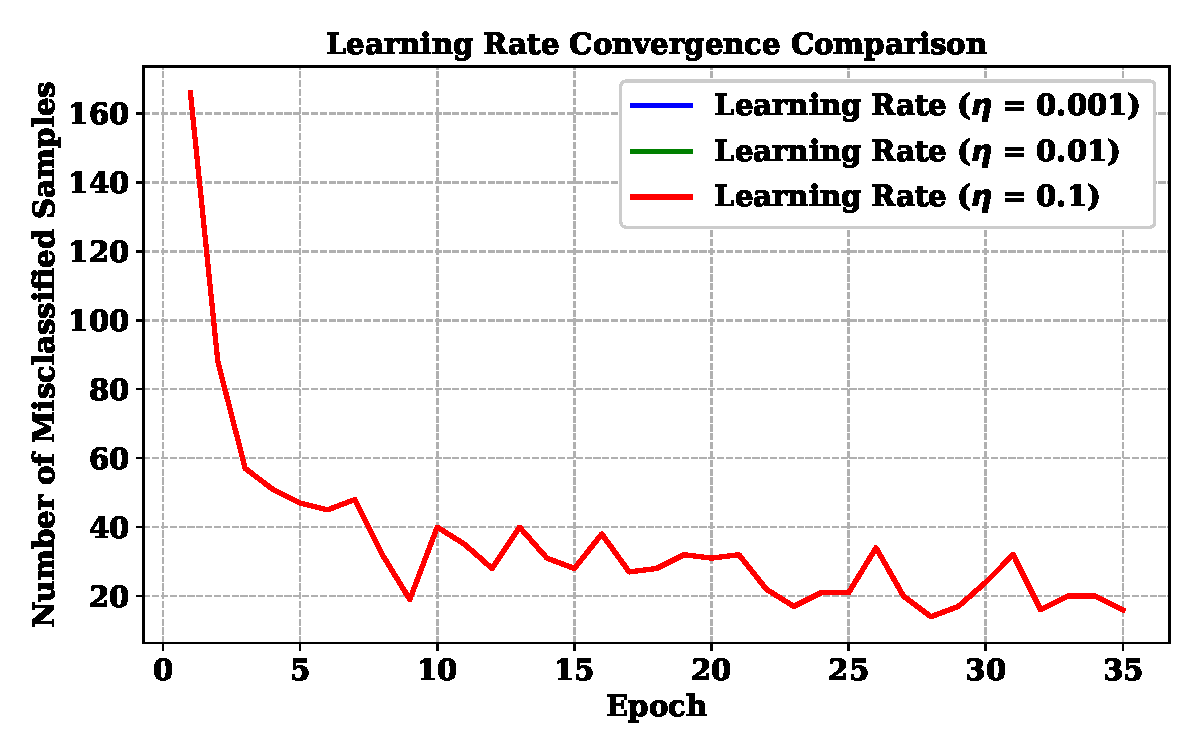
\includegraphics[width=0.7\textwidth]{learning_rate_comparison.eps}
    \caption{Training Error Convergence Profile Across Epochs of different learning rates.}
    \label{fig:learning_rate_comparison}
\end{figure}
\textbf{Interpretation:} All three hyperparameter configurations yield the same error vs epoch curves this is because of the step function which only checks if the input to it crosses the threshold, so even though individual weight values are different we get the same curves.

\begin{figure}[H]
    \centering
    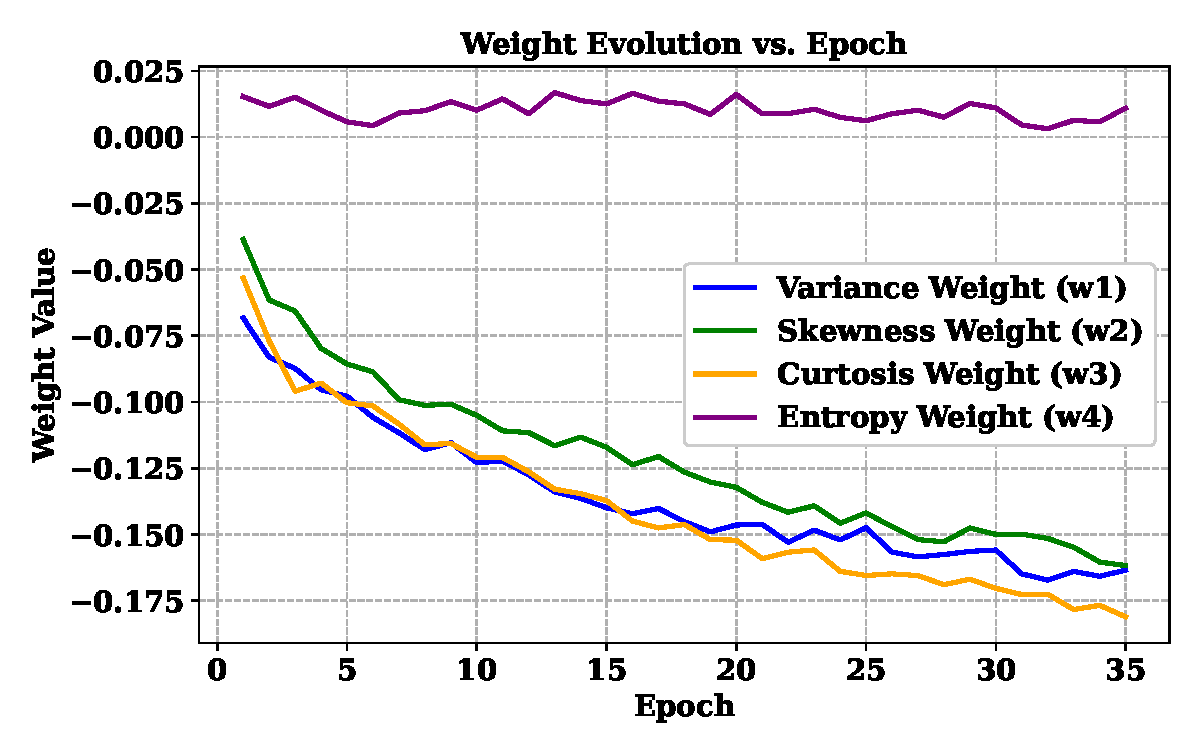
\includegraphics[width=0.7\textwidth]{parameter_evolution.eps}
    \caption{Weight Progression Over Iterations.}
    \label{fig:parameter_evolution}
\end{figure}
\textbf{Interpretation:} As errors move to zero, the weight for Entropy is positive and relatively constant compared to others. All other weights become negative as the number of errors decreases.

\begin{figure}[H]
    \centering
    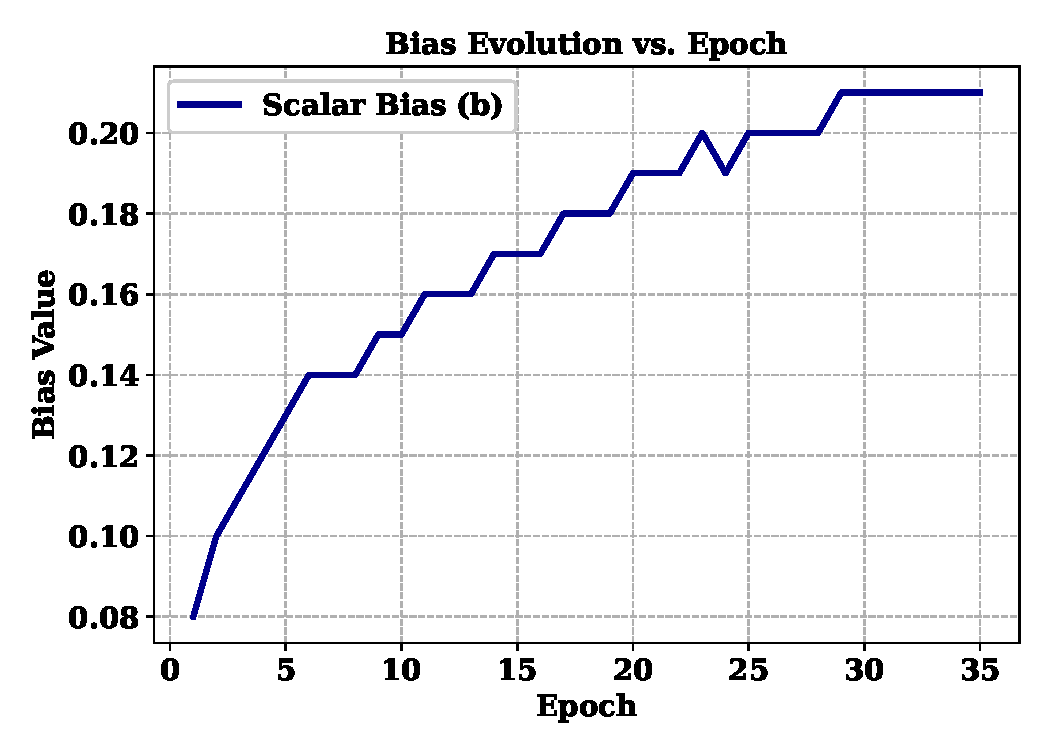
\includegraphics[width=0.7\textwidth]{bias_evolution.eps}
    \caption{Bias Progression Over Iterations.}
    \label{fig:bias_evolution}
\end{figure}
\textbf{Interpretation:} As errors move to zero, the bias increases from zero to about 2.1 and stays constant from there.

\subsection*{Performance Verification}

\begin{figure}[H]
    \centering
    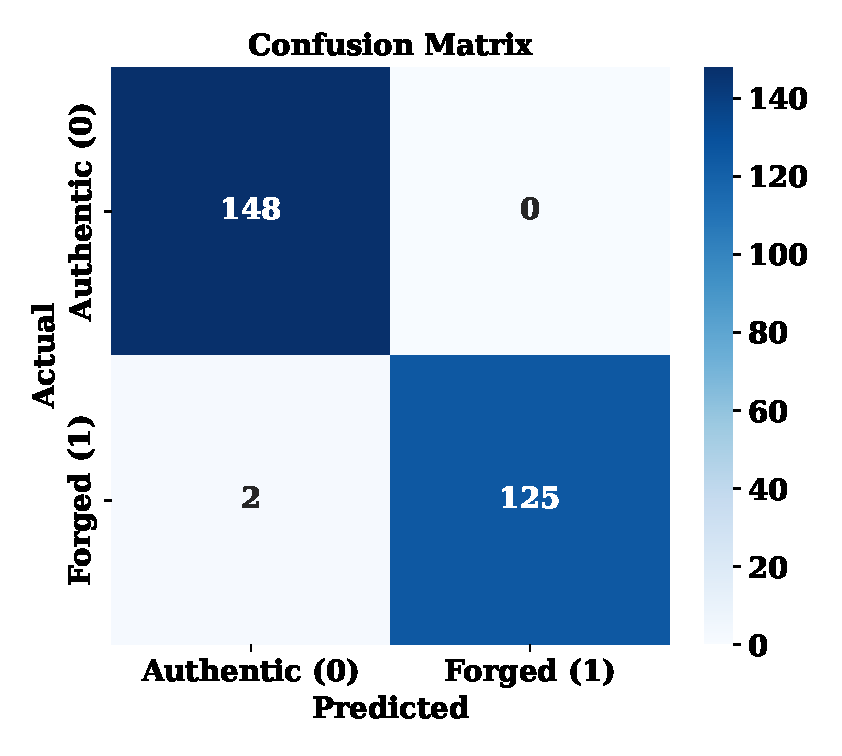
\includegraphics[width=0.7\textwidth]{confusion_matrix.eps}
    \caption{Testing Set Confusion Matrix Heatmap.}
    \label{fig:confusion_matrix}
\end{figure}
\textbf{Interpretation:} There are only 2 false negatives and no false positives. This shows that the model is quite robust for the data.

\begin{figure}[H]
    \centering
    \includegraphics[width=0.7\textwidth]{decision_boundary.eps}
    \caption{Perceptron Decision Boundary.}
    \label{fig:decision_boundary}
\end{figure}
\textbf{Interpretation:} The decision boundary is a line that tries to separate the classes. Since the data here is not fully linearly separable, there are some misclassified points on both sides.

%----------------------------------------------------------

\section*{10. Performance Tables}

\textbf{Training Summary Matrix}
\begin{center}
\begin{tabular}{|p{6cm}|p{7cm}|}
\hline
Dataset Size & 1372 samples \\ \hline
Train/Test Split & 80\% / 20\% \\ \hline
Learning Rate ($\eta$) & 0.01 \\ \hline
Convergence Epochs & 35 \\ \hline
Final Weight Vector ($\mathbf{w}$) & [-0.16, -0.16, -0.18, 0.01] \\ \hline
Final Bias ($b$) & 0.21 \\ \hline
Accuracy & 0.9927 \\ \hline
Precision & 1.0000 \\ \hline
Recall & 0.9843 \\ \hline
F1-score & 0.9921 \\ \hline
\end{tabular}
\end{center}

\vspace{3mm}
\textbf{Epoch-wise Parameter Convergence Log}
\begin{center}
\begin{longtable}{|c|c|c|c|c|c|c|}
\hline
\textbf{Epoch} & \textbf{Errors} & \textbf{Weight 1} & \textbf{Weight 2} & \textbf{Weight 3} & \textbf{Weight 4} & \textbf{Bias}\\ \hline
1 & 166 & -0.07 & -0.04 & -0.05 & 0.02 & 0.08 \\ \hline
7 & 48 & -0.11 & -0.1 & -0.11 & 0.01 & 0.14 \\ \hline
14 & 31 & -0.14 & -0.11 & -0.13 & 0.01 & 0.17 \\ \hline
21 & 32 & -0.15 & -0.14 & -0.16 & 0.01 & 0.19 \\ \hline
28 & 14 & -0.16 & -0.15 & -0.17 & 0.01 & 0.2 \\ \hline
35 & 16 & -0.16 & -0.16 & -0.18 & 0.01 & 0.21 \\ \hline
% Add select key tracking rows from your dataframe logs here
\hline
\end{longtable}
\end{center}

%----------------------------------------------------------

\section*{11. Discussion \& Analysis}

\subsection*{Comparative Study of Activation Functions}
The step function works for the linearly separable data as it just maps one side of the line to class 0 and the other to class 1. However the step function won't be suitable for deep neural networks as it is not differentiable at 0. This is important as deep learning networks rely on the backpropagation which requires the activation function to be differentiable.

\subsection*{Scratch Implementation vs. Scikit-learn Perceptron}
The following results are from the Scikit-Learn perceptron: \\
Accuracy:  0.9418 \\
Precision: 1.0000 \\
Recall:    0.8740 \\
F1-Score:  0.9328 \\

The accuracy and other metrics are lesser than our custom implementation. This difference is because Scikit-Learn's perceptron is an SGDClassifier with a linear loss function. This is different as it uses Stochastic Gradient Descent for optimization and learning whereas the classic perceptron algorithm doesn't.

\subsection*{Hyperparameter Sensitivity (Learning Rate Analysis)}
There was no difference in the convergence plots for the different learning rates provided to the perceptron. The different hyperparameters did change the final weights of the model but the step-function only checks if the weighted-sum of the inputs cross the threshold. In this case the learning rates weren't sensitive enough to cause a difference big enough to cause changes to convergence.

\subsection*{The Linear Separability Constraint (The XOR Problem)}
The XOR problem is a problems that requires a non-linear decision boundary. Perceptrons are only capable of producing a single linear hyperplane. Therefore multi-layer networks are required to produce non-linear decision boundaries to solve problems like the XOR problem.

\subsection*{Impact of Feature Scaling on System Convergence}
Feature scaling makes sure that all the features are on the same scale. This ensures that some weights don't dominate over others leading to better system convergence.

%----------------------------------------------------------

\section*{12. Conclusion}
In this experiment, a Single Layer Perceptron was successfully implemented entirely from scratch to handle real-world binary classification problems, like finding forged banknotes using the Banknote Authentication Dataset.

%----------------------------------------------------------

\section*{13. References}

\begin{enumerate}
\item F. Rosenblatt, ``The Perceptron,'' \emph{Psychological Review}, 1958.
\item I. Goodfellow, Y. Bengio and A. Courville, \emph{Deep Learning}, MIT Press, 2016.
\item C. M. Bishop, \emph{Pattern Recognition and Machine Learning}, Springer, 2006.
\item S. Haykin, \emph{Neural Networks and Learning Machines}, Pearson, 2009.
\item UCI Machine Learning Repository -- Banknote Authentication Dataset.
\item Scikit-learn Documentation: Perceptron.
\end{enumerate}

\end{document}

